\begin{figure}
	
  \setlength{\unitlength}{\textwidth}

  \begin{picture}(1,0.9)(0,0.75)

      % % % Parkinson Data 

      \put(-0.15,0.2){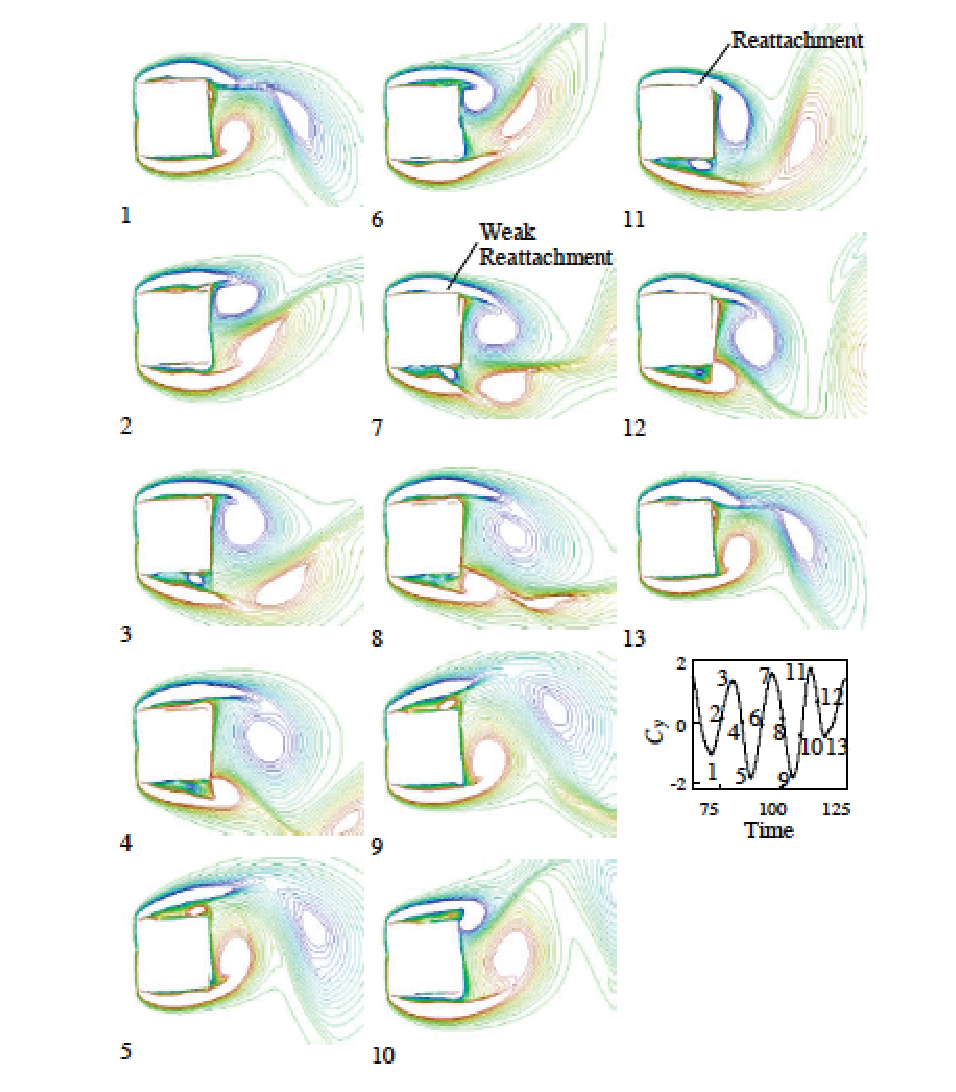
\includegraphics[width=1.3\unitlength]{./chapter-literature-revirw/fnp/luo-re-attachment.eps}}
      
%       \put(0.07,0.95){$\displaystyle\frac{V}{D}$}
%       \put(0.07,1.3){$\displaystyle\frac{A}{D}$}
      
%\put(0.189,1.415){\small(a)}
%\put(0.189,1.07){\small(b)}
%\put(0.189,0.73){\small(c)}

%  


    \end{picture}

  \caption{\label{fig:lit-review-luo-reattachment-1}Vorticity contours of \cy\ and the corresponding time for $\reynoldsnumber=1000$, $\theta=2^{\circ}$ extracted from \citet{Luo2003}. The intermittent shear level is visible in points 7 and 11}
\end{figure}


 %vspace{10cm}
